\documentclass[12pt]{spieman}  % 12pt font required by SPIE;
%\documentclass[a4paper,12pt]{spieman}  % use this instead for A4 paper
\usepackage{amsmath,amsfonts,amssymb}
\usepackage{graphicx}
\usepackage{setspace}
\usepackage{tocloft}
\usepackage{listings}
\lstset{
	numbers=left,
    xleftmargin=2em,
    xrightmargin=1em,
	tabsize=4,
	rulecolor=,
	basicstyle=\scriptsize,
    aboveskip={1.5\baselineskip},
    columns=fixed,
    showstringspaces=false,
    extendedchars=true,
    breaklines=true,
    prebreak = \raisebox{0ex}[0ex][0ex]{\ensuremath{\hookleftarrow}},
    frame=0L,
    showtabs=false,
    showspaces=false,
    showstringspaces=false,
    identifierstyle=\ttfamily,
    keywordstyle=\color[rgb]{0,0,1},
    commentstyle=\color[rgb]{0.133,0.545,0.133},
    stringstyle=\color[rgb]{0.627,0.126,0.941},
    rulecolor=\color{black},
}

\title{Building a containerized ARM Server Farm}

\author[a]{Taylor Chien}
\affil[a]{SUNY Polytechnic Institute, Computer Science Department, 100 Seymour Road, Utica, NY, 13502}

\renewcommand{\cftdotsep}{\cftnodots}
\cftpagenumbersoff{figure}
\cftpagenumbersoff{table} 
\begin{document} 
\maketitle

\begin{abstract}
Open-hardware CPUs have become a major part of our lives, having been integrated into everything from cameras to routers to medical devices. Their simple yet scalable architecture has allowed them to even begin pushing into the enterprise market as a more cost-efficient option for large-scale data analytics. Because of this, the ARM market has stabilized, and server-grade equipment has been edging in on the markets of Intel and AMD. These high-grade ships have even made it back down into Single-Board computers, for the fraction of the cost of an ARM server. This paper is a study of the feasibility of running a containerized environment using these devices.\\


\end{abstract}

\section{Introduction}
\label{sec:intro}
ARM is a low power, open-source CPU architecture that is most commonly found in smart phones, embedded devices, and IoT systems. In the past, ARM was seen as an architecture that could usurp Intel, the king of high-end server processors, and take over data centers. However, with Intel continuing to advance, ARM's focus market divided between licensees, and server-grade ARM processors relatively hard to find, Intel has managed to stay in the data center for now. Qualcomm and Cavium have started edging in with their ARM servers though, targeting multi-threaded workloads with their high core-count, low-power chips. However, one of the biggest breakthroughs for ARM has been that Microsoft recently announced that they would be using ARM CPUs in their Azure cloud service to cut down on costs\cite{microsoftarm}. This is a massive push forward for ARM, and may signmal a greater adoption on the horizon.\\

ARM has also made an impact on the Enterprise market in a very different way. Some high-capacity RAID cards have ARM CPUs on them to help compute parity in a RAID array. ARM also shows up on some manufacturers' Lights-Out Management (LOM) systems. While not a central unit, all of these are important and will generally push ARM along.\\

In the home market ARM has seen the most adoption. Network Attached Storage (NAS) units have seen a massive increase in adoption, due to their low power draw and cheap manufacturing costs, somewhat due to the ARM CPUs most are using. Most consumer-grade routers use either ARM or another open standard, MIPS, as their central processing.\\

The Internet of Things (IoT) is the major push for ARM though. Embedded systems are going to be the next big step for the data center, with small devices branching out from the core, providing backups, fail-over, and distributed workloads. As devices become more integrated, the more chances for them to do work there are. Containerization will allow all of these devices to work at full power as often as they can. Distributed computing between all of these small devices can decentralize a data center to prevent single points of failure.\\

So far, the most popular ARM device is the Raspberry Pi. This small, \$35 computer was developed by a British non-for-profit. Over a million Raspberry Pis have been sold so far, and the device has even made it on board the ISS as part of public research projects. The Raspberry Pi was such a hit, that when their first run of the extremely small Raspberry Pi Zero was put up for sale, it sold out from most retailers in hours. Because of its simplicity and great documentation, it has become the device that all other have had to measure up to.\\

However, the Raspberry Pi isn’t alone anymore. Competitors for other niche markets such as industrial systems, embedded servers, kiosks, and even desktops have popped up. Some of the devices out there contain the same CPUs that run high-end servers, while others pull so little power they can run off a solar panel.\\

Enterprise ARM devices are still expensive and hard to find due to their relatively new arrival on the market. On the other hand, consumer devices are now cheaper than ever. If ARM is still set to become the next big thing, testing it on these consumer devices will more than demonstrate the advanced features that the Enterprise chips can match, and at a fraction of the cost.\\

\section{Literature Review}
\label{sec:lit-rev}

The original inspiration for this project came from Jeff Geerling's Raspberry Pi Dramble\cite{geerlingdramble}, where he uses Ansible to set up a small cluster of Raspberry Pis into a miniature web service with fail-over. He had a fully redundant cluster of Raspberry Pis, with a load balancer, web servers, and a fail-over enabled MySQL server. This is a full production environment, available from anywhere on the Internet. This is still running on the bare metal though, not in a containerized system, which is where I wanted to focus.\\

This problem was solved by looking at a group\cite{hypriotkubernetes} who set up Kubernetes, a distributed containerization system, on a bunch of Raspberry Pis and developed a port of the operating system for it. This allows all the redundancy and fail-over of a normal data center, only with devices that pull power measured in watts, not kilowatts. Distributing this cluster around a campus or throughout different cities would allow a fail-over mesh of unprecedented reliability, especially with distributed file systems and these cheap, simple devices.\\

Another inspiration came when searching for ARM-powered enterprise devices, such as Cavium's Thunder-X chips. Gigabyte and System76 sell this chip in blade and rack-mount servers. While looking at comparisons of these, I found an article about how Intel bought the Thunder-X version of the Gigabyte server that their Xeon chips run in and ran benchmarks comparing the two\cite{morganarmxeon}. ARM and Intel's x86 are by definition different architectures, and what the tests showed was in what areas each excels. In multi-threaded workloads, the ARM chips were better, but for time-sensitive or latency-sensitive tasks, the x86 server won, since ARM doesn't have a Layer 3 cache.\\

Towards the end of the article, the author lists the reason that ARM isn't as fast; Intel has been pushing for usability, adding features and technologies that boost performance and features, such as Thunderbolt, DDR4 support, L3 cache, better single-core performance, core sharing, and Hyperthreading (semi-virtual CPU cores). ARM on the other hand has been fixing their base features and trying to conglomerate their fractured platform into a more solid competitor. This is slowly but steadily starting to show, as new ARM chips can press 48 or more cores into a single die. However, Intel is starting to get in on the low-powered, high-core-count market with their Phi CPU lineup, which features up to 64 cores and 256 threads of lower-speed processing power\cite{linus64xeon}.\\

\section{Methods and Materials}
\label{sec:met-mat}
\subsection{Devices}
\label{subsec:arm-groups}

For this test, a reliable platform was needed. In the end, the Odroid XU4 variants (HC1 for storage, and MC1 for compute) were chosen due to their great CPU power and multitude of CPU Cores. The Odroid XU4 has 2 GB of RAM, gigabit Ethernet, and a Samsung Exynos 5422 eight-core heterogeneous CPU, with four cores running the 2.4GHz ARM A15 architecture, and four running the 1.4GHz A7 architecture. By comparison, the Raspberry Pi runs 1 GB RAM, fast Ethernet, and a Broadcom BCM2837 quad-core A53 1.2GHz CPU. While both have been vetted by extensive testing and personal experience, the Odroid crushes the Raspberry Pi in the performance department. The MC1s and HC1s also come with already-built case and heat sink, which boosts them above the Raspberry Pi again, since that needs a separate case and heat sink.\\

The MC1 and HC1 variants of the Odroid XU4 are specialized for two different purposes. The HC1s are specialized for storage, with an integrated SATA header and mount points on the chassis for a 2.5" hard drive or SSD. Easily capable of running some of the more demanding distributed file systems out there, like Ceph and GlusterFS, the HC1 is perfect for running the storage of this network. The MC1 is intended for compute purposes, since it is sold in pre-assembled groups of four, these groups are meant to run computations.

\begin{table}[ht]
\caption{Comparison of ARM Devices} 
\label{tab:device-analysis}
\begin{center}       
\begin{tabular}{|l|l|l|l|l|l|}
\hline
\rule[-1ex]{0pt}{3.5ex}  Device & Quantity & CPU Cores & RAM (GB) & Total CPUs & Total RAM (GB) \\
\hline\hline
\rule[-1ex]{0pt}{3.5ex}  Odroid MC1 & 80 & 8 & 2 &  640 & 160 \\
\hline
\rule[-1ex]{0pt}{3.5ex}  Odroid HC1 & 20 & 8 & 2 &  160 & 40 \\
\hline
\rule[-1ex]{0pt}{3.5ex}  Total & - & - & - & 800 & 200 \\
\hline
\end{tabular}
\end{center}
\end{table} 

\subsection{Device Usage}
\label{subsec:arm-usage}

The main computational power of the network will come from the MC1 devices, which will be used for running the containerization software itself. Because of the raw computational power of the Samsung ARM CPU, these devices are capable of some truly amazing power. With their newer, more capable heatsink, the bottleneck that plagued the XU4 platform is now gone.\\

On the storage side, twelve HC1s will be used to run Ceph, a distributed storage solution. They will be divided into three stacks, with each one linked to an MC1 pool physically to share the power and storage. Overall, all these storage devices will be linked virtually to share and distribute the workload of the ceph cluster.\\

Some devices will be acting outside of the main compute and storage groups, in order to allow other services to run without using the main pools of devices. The first group will be for the core services, such as DNS, LDAP, phpldapadmin, an OpenVPN Server, and UPS monitoring software. This will be handled by two of the MC1 clusters, using load-balancing features within Linux to keep the services alive at all times. In total, there will be eight devices working on core services, likely on separate physical segments to prevent a single point of failure.\\

The second group will be for backups. Four of the HC1s will be pooled with GlusterFS and used to back up configuration files and containers. Again, they will likely be on different network segments to prevent a single point of failure.\\

Another special group will have two HC1s running the package repository for the operating system. To keep traffic through the external connection as low as possible, a mirror will be set up internally to allow the packages to be updated from the inside. This will both speed up access to the packages themselves, and allow the network to operate without the bandwidth hit of having a hundred devices updating all at once.

\subsubsection{MC1 Compute Pools}
\label{subsubsec:arm-usage-mc1-compute}

The pools will be labeled A, B, and C to differentiate between them physically. Each pool will contain three master nodes, one in every other stack. This means a total of nine masters, each managing seven servers. With the amount of power available, other compute options are available, such as minor virtualization, distributed computing, or even blockchain mining. The most likely options are Kubernetes and Docker Swarm, which will allow for several hundred containers to be run at once.

\subsubsection{HC1 Storage Cluster}
\label{subsubsec:arm-usage-hc1-storage}

The HC1s will be set up in a Ceph pool that covers all three of the MC1 pools with unified storage. The Ceph pool will be split in half physically, meaning each half will be on a separate physical segment of the network. There will only be two physical pools, A and B, but it will allow the pool to be mirrored across two branches of the network. 

\subsubsection{Core Devices}
\label{subsubsec:arm-usage-core}

The core devices will be split into two separate physical stacks to help keep them redundant. Each stack of four devices, with each device running a small set of services, which will be kept alive using LinuxHA or similar load balancing method.\\

\textbf{Device 1:} bind9 Provider, openldap Provider; Does not serve requests, only acts as master\\

\textbf{Device 2:} bind9 Consumer, openldap Consumer, phpLDAPadmin\\

\textbf{Device 3:} bind9 Consumer, openldap Consumer, UniFi controller\\

\textbf{Device 4:} bind9 Consumer, openvpn, and ssh server, nutd server (UPS Monitoring)\\

\subsubsection{Backups Storage}
\label{subsubsec:arm-usage-backups}

All backups on the network will be handled by four HC1s, pooled with GlusterFS and using a program like Bacula to automate the backup process. Because the pool won't have as much storage as the main Ceph pool, not everything will be backed up. Configurations, the core image, and some containers are likely to be the main candidates.\\

This pool will also be running a syslog server to pull logs from the entire cluster. These will be kept on a seperate chunk of the GlusterFS pool to prevent the logs from taking up all the space. logrotate will be used to compress and move the daily logs to the backup directory to prevent their loss.

\subsubsection{Repository Storage}
\label{subsubsec:arm-usage-repo}

The repository server will contain a clone of the armhf Debian repository, synced using the method Debian recommends for creating personal repositories. These HC1s will also have the same 4 TB drives that the backup servers have, allowing them to hold the repository. Other repositories might be added later, such as the Docker repository, since there is plenty of space. GlusterFS replication will be used to ensure no data is lost, and that the web site is accessible from either device at any time, and that both devices can split the load of downloading additional Debian packages.

\subsection{Storage}
\label{subsec:arm-storage}

Each device will be using a 16 GB Class 10 microSD Card as the boot drive. While EMMC is faster, it is also more expensive and more difficult to work with. microSD will work for what we need it for, and is fast enough.\\

The Ceph HC1s will each have a WD Black 1 TB 2.5" hard drive connected to their SATA port. These drives will be the dedicated Ceph storage for all the nodes, and will be more than enough for this network.\\

The other six HC1s will be using Seagate Barracuda 4 TB 2.5" hard drives. These drives are slower, but their usage won't require that speed, only the capacity they offer.

\subsection{Power}
\label{subsec:arm-power}

Because all of these devices are the same voltage, a very simple power solution can be used. Switching power supplies for LED strips can deliver more than enough power for these devices to run. Up to 300 Watts worth of power can be pulled from each power supply. The only issue with these devices is that they have to be wired manually, since they are meant to be wired directly to the mains power.\\

Each of the MC1 pools will be split in two, and each half will connected to one power supply. Each half of the HC1 Ceph pool will connect to one supply. One core stack, one repository device, and one half of the backup pool will each share a power supply as well. This comes out to ten of these power supplies, for a total of 3,000 Watts of power. \\

In addition, there will be two 1500VA UPSes, each capable of powering five of the power supplies in case of an outage, as well as smoothing the power. These will alert two of the core service devices when there is a power outage so that they can begin shutting down devices as needed until power is restored.

\subsection{Operating System}
\label{subsec:arm-os}

For this project, using the same operating system across all devices was important to maintain a common base for all devices. CentOS and Fedora have limited ARM support, so they were skipped over. Ubuntu has the same issue. However, Debian supports ARM fully, and there are many ports just for ARM. This, however, has its own problem. While these ports are Debian at their core, there are some very critical changes.\\

The two main contenders are Armbian and DietPi. Each was built with a different intended use, so they are somewhat changed from Core Debian, changing how they perform under the high stress of full load.\\

Armbian was developed to unify as many open ARM platforms as possible and enable them to use the same libraries and repositories. However, it was really meant for IoT and light server usage, not enterprise functionality. There are often issues, and bugs are rampant throughout the system. Also, some Armbian packages are set to overwrite existing files instead of asking, and some kernel modules and packages are installed by default and can’t be removed without recompiling the kernel. This wouldn't be a problem if their compiler tool worked, but often the build process contains numerous issues that break what is being compiled. Some devices may have several available kernels under different operating systems available, while others will only have a single kernel without another operating system choice.\\

On the other hand, DietPi is meant to make server setup a breeze, which causes issues when first using the device, if all you want is a terminal. It also does not have the massive amount of bloat when it starts as Armbian, but it also contains less of the core services overall, although their manu system is actually very easy to navigate once it is understood.\\

In the end, DietPi was chosen due to how close it is to Debian, and how much support the developers built in, even if the OS itself starts out a little light.

\subsection{Networking}
\label{subsec:arm-network}

Because there are so many devices, multiple switches are needed. The 24-port \\

There will be five VLANs overall; one for the MC1 devices, one for the HC1 devices, one for the VPN server to park clients on, one for containers and virtual IPs, and a disconnected "parking" VLAN for unused devices.

\subsection{Configuration}
\label{subsec:arm-config}

Because there are so many devices, getting all of the configurations out will be next to impossible. This is where a mixture of two configuration methods comes in. All of the methods will have their specific configurations combined on Github, which will allow them to be updates as they are needed.

\subsubsection{Bash Scripts}
The first item that will be run is a set of custom bash scripts aimed at turning the default, vanilla installation of Debian into a more custom variant. These scripts will be used to set common items, like the host name, motd, SSH server configuration, IP address, DNS servers, startup services, kernel modules, and some basic configurations. It will also install the common packages that are needed, as well as generating basic scripts for other tasks, like SSH Host Key regeneration and firewall rules.\\

Some of the major elements of this script will be to:
\begin{itemize}
\item Identify the system based on MAC address or Serial Number, using a pre-compiled list of all devices.
\item Generate static text files using the information found during device discovery, such as hostname, stack location, IP Address, and MAC. This information will be used to create files like the MOTD, SSH Banner, and /etc/issue.
\item Generate common configurations for services, namely SSHD, sysctl, networking, iptables, sssd, apt, and ntp. These will mostly be default across all devices, with specifics changed by later configuration methods as needed.
\item Install programs like vim, sudo, iptables-persistent, fail2ban, and others, then configure those as well.
\item Add essential items, like SSH Keys, .bashrc, .screenrc, .vimrc, and system-wide bash.bashrc and default shells.
\item Set correct root and user passwords, and restrict the use of Sudo and Su.
\end{itemize}

\subsubsection{Ansible}
The second method is Ansible, a configuration utility based around pre-built "playbooks" being run over SSH. Ansible playbooks aren't commands, but are used to manage systems through SSH. This will be used to break the systems into the groups defined above. Because Ansible only executes commands over SSH, it doesn't need to have a piece of software on the remote side to connect to. It executes the commands on the remote system in a pattern defined by the playbook.\\

The hosts will be grouped based on their tasks, with some hosts being included in multiple groups, such as the Docker and Docker Swarm Master groups, as well as Pool and Stack specific groups.\\

Ansible will mostly be responsible for the following:
\begin{itemize}
\item Installing specific packages for services, such as Docker, GlusterFS, or any others.
\item Configuring services on a per-system basis, such as extra network interfaces, load balancing, any system configuration.
\item Pass configuration files, scripts, and images to individual server groups.
\end{itemize}


\subsection{Physical Device Setup}
\label{subsec:arm-physical-setup}

\begin{figure}[H]
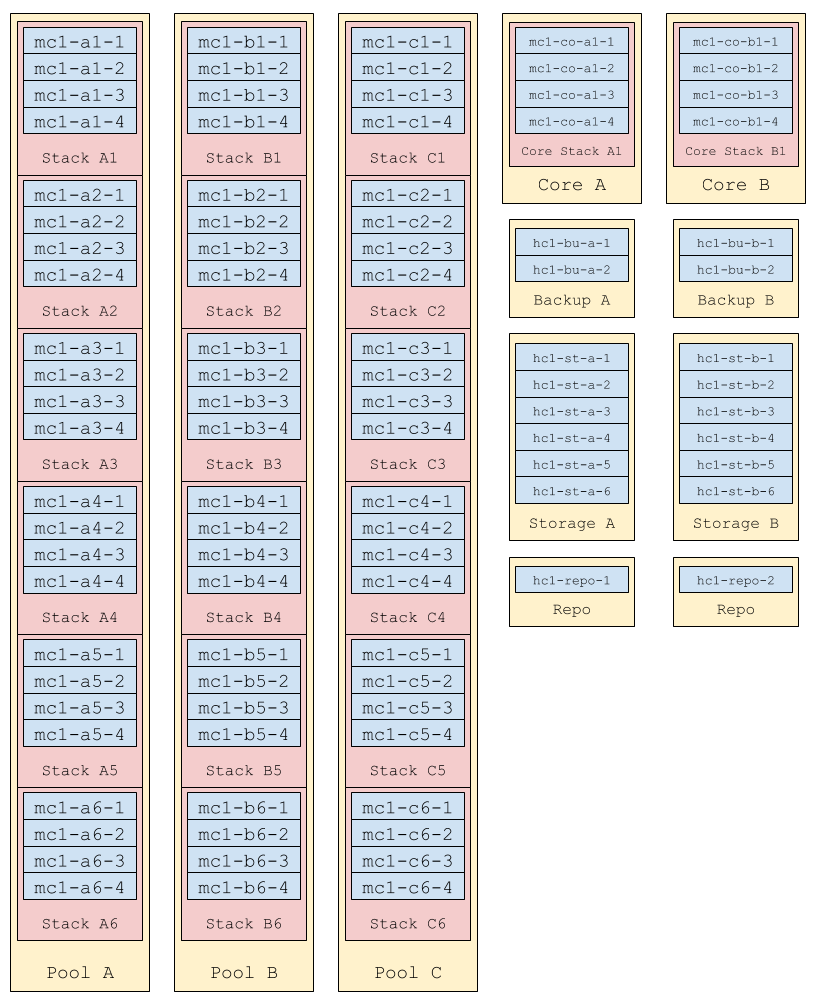
\includegraphics[width=14cm]{images/Pool_Map.png}
\centering
\label{img:pool-map}
\caption{Map of Physical Device Organization. Pools A, B, and C are for Docker Swarm, with the first node being the master. The HC1s, while virtually pooled, will be physically separated for power reasons}
\end{figure}



\section{Results}
\label{sec:results}


\section{Discussion}
\label{sec:discussion}

ARM itself may be a relatively cheap and useful platform, but it is fractured. Many of the features and capabilities are split across multiple generations, and the software has done the same.

\section{Conclusion}
\label{sec:conclusion}


% \begin{figure}
% \begin{center}
% \begin{tabular}{c}
% \includegraphics[height=5.5cm]{mcr3b.eps}
% \end{tabular}
% \end{center}
% \caption {Picture}
% \label{fig:example}
% \end{figure}

\appendix
\acknowledgments 
I would like to thank Professors Joshua White and Ali Tekeoglu from SUNY Polytechnic Institute for supporting this project and checking my paper. I would also like to thank the SUNY Polytechnic's CSTEP Program, NCS Club, Computer Club, Computer Science Department, and DogNet for providing moral and minor material support. Special thanks goes to Marissa Kitts and Luke Kunz for offering edible assistance (they brought me food).

%%%%% References %%%%%

\bibliography{report}   % bibliography data in report.bib
\bibliographystyle{spiejour}   % makes bibtex use spiejour.bst

\end{document}